\documentclass[tikz,border=8pt]{standalone}
\usepackage[scaled=0.95]{helvet}
\renewcommand{\familydefault}{\sfdefault}
\usepackage[europeanresistors,americanvoltages]{circuitikz}
\definecolor{TEJNavy}{HTML}{1E2B55}
\definecolor{TEJBlue}{HTML}{1769AA}
\definecolor{TEJOrange}{HTML}{E97828}
\begin{document}
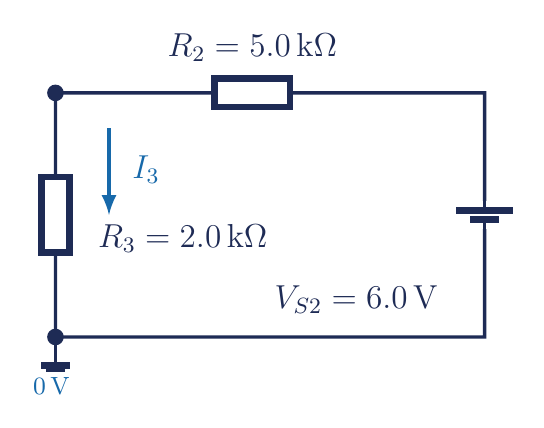
\begin{tikzpicture}[line width=1.2pt,draw=TEJNavy,text=TEJNavy,>=latex]
  \ctikzset{bipoles/length=1.2cm}

  % Canonical isolated Loop 2 topology.
  \draw (0.9,3.9)
    to[R] (0.9,0.8)
    -- (6.35,0.8)
    to[battery1,invert] (6.35,3.9)
    -- (4.65,3.9)
    to[R] (2.15,3.9)
    -- (0.9,3.9);
  \draw (0.9,0.8) node[ground] {};
  \fill[TEJNavy] (0.9,3.9) circle (3pt);
  \fill[TEJNavy] (0.9,0.8) circle (3pt);

  \node[fill=white,inner sep=2pt,font=\large] at (3.40,4.48)
    {$R_2=5.0\,\mathrm{k}\Omega$};
  % Anchor branch labels away from their wires so no glyph crosses a conductor.
  \node[fill=white,inner sep=2pt,font=\large,anchor=east] at (5.85,1.28)
    {$V_{S2}=6.0\,\mathrm{V}$};
  \node[fill=white,inner sep=2pt,font=\large,anchor=west] at (1.35,2.05)
    {$R_3=2.0\,\mathrm{k}\Omega$};
  \node[fill=white,inner sep=2pt,font=\small,text=TEJBlue] at (0.85,0.18)
    {$0\,\mathrm{V}$};

  % One current cue only, beside the shared resistor.
  \draw[->,TEJBlue,line width=1.45pt] (1.58,3.45) -- (1.58,2.35);
  \node[fill=white,inner sep=2pt,font=\large,text=TEJBlue] at (2.05,2.92)
    {$I_3$};
\end{tikzpicture}
\end{document}
